\chapter{СОСТАВЛЕНИЕ МАТЕМАТИЧЕСКОЙ МОДЕЛИ ПНЕВМОПРИВОДА}\label{ch:ch2}
Данная глава посвящена математическому моделированию ПП
с дискретными распределителями. Рассматриваются следующие ключевые аспекты:

\begin{enumerate}
    \item Структура и принцип работы исследуемого ПП;
    \item Моделирование пневмоцилиндра;
    \item Моделирование дискретных распределителей;
    \item Моделирование силы трения и упругих деформаций;
    \item Адаптация математической модели к эффективному численному расчету на ЭВМ.
    \item Верификация математической модели.
\end{enumerate}

Математическая модель включает:

\begin{enumerate}
    \item Уравнения движения поршня;
    \item Уравнения изменения давления в полостях цилиндра;
    \item Уравнения изменения температуры рабочего тела в полостях цилиндра;
    \item Модель массового расхода воздуха;
    \item Модель динамики распределителей;
    \item Модель сил трения;
    \item Модель силы реакции опоры.
\end{enumerate}

Используются уравнения термодинамики и газовой динамики. Учитываются нелинейные эффекты:
сжимаемость воздуха, особенности течения через дросселирующие элементы, силы трения и реакции опоры.

Верификация модели проводится путем проверки математической корректности.



\section{Структура и паринцип работы исследуемого пневмопривода}\label{sec:ch2/sec1}

Исследуемый электропневматический привод включает пневматический цилиндр двустороннего действия
c односторонним штоком и четыре двухпозиционных распределителя.
Цилиндр содержит две рабочие полости, разделенные поршнем.

Ключевой особенностью привода является конфигурация распределителей.
К каждой полости цилиндра подключены два независимых распределителя:
один для подачи сжатого воздуха из магистрали, другой для выхлопа в атмосферу.
Такая конфигурация обеспечивает гибкое управление потоками воздуха в обеих полостях цилиндра.

[Рисунок: Принципиальная пневматическая схема привода с указанием подключения распределителей]

Каждый распределитель имеет два дискретных состояния: открыто и закрыто.
Общее количество возможных комбинаций состояний распределителей
определяется формулой:
\begin{equation*}
    N = 2^k,
\end{equation*}
где $N$ - число комбинаций, $k$ - количество распределителей.

Для рассматриваемой системы с четырьмя распределителями:
\begin{equation*}
    N = 2^4 = 16.
\end{equation*}

Таким образом, система имеет 16 дискретных состояний, что обеспечивает широкие возможности
управления при сохранении относительной простоты конструкции.

Система управления генерирует дискретные сигналы для активации
электромагнитных клапанов распределителей. Обратная связь по положению реализуется посредством датчика линейного перемещения на штоке цилиндра. Дополнительно могут применяться датчики давления в полостях цилиндра для повышения точности управления.

[Рисунок: Функциональная схема системы управления приводом]

Использование дискретных распределителей вместо пропорциональных
снижает стоимость системы, однако требует разработки более сложных
алгоритмов управления для компенсации нелинейного характера коммутации пневматических линий.

\section{Моделирование пневмоцилиндра}\label{sec:ch2/sec2}

При разработке математической модели пневмоцилиндра были приняты следующие основные допущения:
\begin{enumerate}
    \item Рабочим телом является идеальный газ (воздух), подчиняющийся уравнению состояния Клапейрона-Менделеева;
    \item Процессы в рабочих полостях пневмоцилиндра рассматриваются как адиабатические, теплообмен с окружающей средой не учитывается;
    \item Температура газа в магистрали и температура окружающей среды принимаются постоянными;
    \item Утечки газа через уплотнения поршня и штока не учитываются;
    \item Давление в выхлопной магистрали принимается равным атмосферному;
    \item Влияние сил тяжести на движение поршня не учитывается ввиду горизонтального расположения пневмоцилиндра;
    \item Пневматические линии между распределителями и рабочими полостями цилиндра считаются короткими,
          их объем пренебрежимо мал по сравнению с объемом рабочих полостей;
    \item Эффекты сжимаемости воздуха в трубопроводах не учитываются.
\end{enumerate}

С учетом принятых допущений, математическая модель пневмоцилиндра может быть представлена системой
дифференциальных уравнений, описывающих изменение давлений в рабочих полостях, температур газа и
движение поршня. Данная система уравнений формирует основу для дальнейшего анализа динамики пневмопривода
и синтеза алгоритмов управления.

\subsection{Уравнение движения пневмоцилиндра}\label{sec:ch2/sec2/subsec1}

Рассмотрим пневмоцилиндр как систему с одной степень свободы. Обобщенной координатой выберем положение поршня $x$.
Для применения принципа Гамильтона необходимо составить функцию Лагранжа:
\begin{equation}\label{eq:ch2/eq0}
    L = T - U,
\end{equation}
где $T$ -- кинетическая энергия системы; $U$ -- потенциальная энергия системы; $L$ -- функция Лагранжа.

Кинетическую энергию системы можно представить в виде:
\begin{equation}\label{eq:ch2/eq1}
    T = \frac{M}{2} \dot{x}^2,
\end{equation}
где $M$ -- масса подвижных частей системы; $\dot{x}$ -- скорость движения поршня.

Потенциальная энергия системы включает в себя работу силы давления газа в рабочих полостях цилиндра:

\begin{equation}\label{eq:ch2/eq2}
    U = p_1 V_1 + p_2 V_2 + p_\text{атм} (V_1 - V_2),
\end{equation}
где $p_1$ и $p_2$ -- давления в рабочих полостях цилиндра;
$V_1$ и $V_2$ -- объемы рабочих полостей;
$p_\text{атм}$ -- атмосферное давление.

Объемы рабочих полостей связаны с положением поршня следующим образом:
\begin{equation}\label{eq:ch2/eq3}
    \begin{aligned}
        V_1 & = F_1 (x - x_0),     \\
        V_2 & = F_2 (L - x + x_0),
    \end{aligned}
\end{equation}
где $F_1=\pi D_{поршня}^2/4 $ и $F_2 = \pi (D_{поршня}^2/4 - D_{штока}^2/4)$ -- активные площади поперечного сечения поршня в поршневой и штоковой полостях соответственно;
$x_0$ -- начальное положение поршня;
$L$ -- ход поршня.

Подставляя \eqref{eq:ch2/eq1}, \eqref{eq:ch2/eq2} и \eqref{eq:ch2/eq3} в \eqref{eq:ch2/eq0}, получим функцию Лагранжа:

\begin{equation}\label{eq:ch2/eq4}
    \begin{aligned}
        L & = \frac{M}{2} \dot{x}^2 - p_1 F_1 (x - x_0) - p_2 F_2 (L - x + x_0) \\
          & - p_\text{атм} (F_1 (x - x_0) - F_2 (L - x + x_0)).
    \end{aligned}
\end{equation}

Обобщенную силу $Q_x$, действующую на систему учитывющую силу трения и реакции упоров, можно представить в виде:
\begin{equation}\label{eq:ch2/eq5}
    Q_x = - R_{\text{тр}} - R_{\text{упор}},
\end{equation}
где $R_{\text{тр}}$ -- сила трения; $R_{\text{упор}}$ -- сила реакции упора.

Запишем уравнение лагранжа в общем виде:

\begin{equation}\label{eq:ch2/eq6}
    \frac{d}{dt} \left( \frac{\partial L}{\partial \dot{x}} \right) - \frac{\partial L}{\partial x} = Q_x.
\end{equation}

Вычислим частные производные функции Лагранжа \eqref{eq:ch2/eq4} по обобщенной координате $x$ и ее производной $\dot{x}$:

\begin{equation}\label{eq:ch2/eq7}
    \begin{aligned}
        \frac{\partial L}{\partial \dot{x}} & = M \dot{x},                                    \\
        \frac{\partial L}{\partial x}       & = p_1 F_1 - p_2 F_2 - p_\text{атм} (F_1 - F_2).
    \end{aligned}
\end{equation}

Подставляя \eqref{eq:ch2/eq7} и \eqref{eq:ch2/eq5} в \eqref{eq:ch2/eq6}, получим уравнение движения пневмоцилиндра:

\begin{equation}\label{eq:ch2/eq8}
    M \ddot{x} = p_1 F_1 - p_2 F_2 - p_\text{атм} (F_1 - F_2) - R_{\text{тр}} - R_{\text{упор}}.
\end{equation}
где $\ddot{x}$ -- ускорение поршня.

\subsection{Уравнения изменения давлений в полостях пневмоцилиндра}\label{sec:ch2/sec2/subsec2}

Первоначально получим дифференциальные уравнения изменения давлений в
полостях пневмоцилиндра, основываясь на началах термодинамики
и уравнения Максвелла с учетом ранее принятых допущений.
Ключевыми допущениями для данного вывода являются: рассмотрение
воздуха как идеального газа, адиабатический характер процессов в полостях
цилиндра, отсутствие утечек газа через уплотнения, и пренебрежение объемом
пневматических линий между распределителями и рабочими полостями.

Согласно первому началу термодинамики для открытой системы, изменение внутренней энергии рабочего тела
описывается уравнением:

\begin{equation}
    dU = \partial Q - \partial W + hdm,
\end{equation}
где $dU$ - изменение внутренней энергии;
$δQ$ -- подведенное тепло;
$δW$ -- совершенная работа;
$h$ -- удельная энтальпия;
$dm$ -- изменение массы системы.

Учитвая, что процесс рассматривается как адиабатический, то $δQ = 0$ и
работа совершается только за счет изменения объема газа в полостях цилиндра:

\begin{equation*}
    \partial W = -pdV.
\end{equation*}

Тогда уравнение изменения внутренней энергии примет вид:

\begin{equation*}
    dU = -pdV + hdm.
\end{equation*}

Используя определение энтальпии $H - U = pV$, получим:

\begin{equation*}
    d(H-pV) = -pdV + hdm.
\end{equation*}

Раскрывая дифференциалы, получим:

\begin{equation*}
    dH - pdV - Vdp = -pdV + hdm.
\end{equation*}

Сокращая слагаемые, получим уравнение изменения энтальпии:

\begin{equation}\label{eq:ch2/eq9}
    dH = Vdp + hdm.
\end{equation}

Выражение \eqref{eq:ch2/eq9} позволяет описать изменение энтальпии рабочего тела в процессе сжатия и
расширения, а также в при изменении массы рабочего тела.

Обратися к уравнению Максвелла для энтальпии, которое связывает изменение энтальпии с изменением давления и температуры:

\begin{equation}\label{eq:ch2/eq10}
    dH = \left(
    \frac{\partial H}{\partial p}
    \right)_T dp + \left(
    \frac{\partial H}{\partial T}
    \right)_p dT.
\end{equation}

Приравнивая правые части уравнений \eqref{eq:ch2/eq9} и \eqref{eq:ch2/eq10}, получаем:

\begin{equation}\label{eq:ch2/eq11}
    \left(
    \frac{\partial H}{\partial p}
    \right)_T dp + \left(
    \frac{\partial H}{\partial T}
    \right)_p dT = Vdp + hdm.
\end{equation}

На данном этапе воспольуемся одним из соотношений Максвелла:

\begin{equation*}
    \left(
    \frac{\partial H}{\partial p}
    \right)_T = V - T \left(
    \frac{\partial V}{\partial T}
    \right)_p.
\end{equation*}

Подставляя это выражение в \eqref{eq:ch2/eq11}, получим:

\begin{equation*}
    \left( V - T \left(
        \frac{\partial V}{\partial T}
        \right)_p \right) dp + \left(
    \frac{\partial H}{\partial T}
    \right)_p dT = Vdp + hdm.
\end{equation*}

После упрощения и группировки членов, приходим к следующему выражению:
\begin{equation}\label{eq:ch2/eq12}
    -T \left(
    \frac{\partial V}{\partial T}
    \right)_p dp + \left(
    \frac{\partial H}{\partial T}
    \right)_p dT = hdm.
\end{equation}

Здесь можно воспользоваться еще одним важным термодинамически соотножениемЖ
\begin{equation}\label{eq:ch2/eq13}
    \left(
    \frac{\partial H}{\partial T}
    \right)_p = c_p,
\end{equation}
где $c_p$ -- удельная теплоемкость при постоянном давлении.

Подставляя \eqref{eq:ch2/eq13} в уравнение \eqref{eq:ch2/eq12}, получим:
\begin{equation}\label{eq:ch2/eq14}
    -T \left(
    \frac{\partial V}{\partial T}
    \right)_p dp + c_p dT = hdm.
\end{equation}

Для идеального газа справедливо соотношение:

\begin{equation*}
    \left(\frac{\partial V}{\partial T}\right)_p = \frac{R}{p},
\end{equation*}
где $R$ -- газовая постоянная.

Используя данное выражение, преобразуем уравнение:

\begin{equation*}
    -\frac{RT}{p} dp + c_p dT = h dm.
\end{equation*}

Разделив обе части на $dt$ и учитывая, что $dm/dt = G$ (массовый расход), получаем дифференциальное уравнение:

\begin{equation*}
    -\frac{RT}{p} \frac{dp}{dt} + c_p \frac{dT}{dt} = hG.
\end{equation*}

Теперь обратимся к уравнению состояния идеального газа $pV = mRT$. Дифференцируя его по времени, получаем:

\begin{equation*}
    V\frac{dp}{dt} + p\frac{dV}{dt} = RT\frac{dm}{dt} + mR\frac{dT}{dt}.
\end{equation*}

Подставляя выражение для $dT/dt$ из предыдущего уравнения и учитывая, что для идеального газа

\begin{equation*}
    c_p - c_v = R,
\end{equation*}
где $c_v$ -- удельная теплоемкость при постоянном объеме, после ряда алгебраических преобразований получаем:

\begin{equation}\label{eq:ch2/eq15}
    \frac{dp}{dt} = \frac{\gamma}{V}\left(RT\frac{dm}{dt} - p\frac{dV}{dt}\right),
\end{equation}
где $\gamma = c_p/c_v$ -- показатель адиабаты.

Теперь учтем, что к каждой полости пневмоцилиндра подключены два независимых распределителя:
один для подачи сжатого воздуха из магистрали, другой для выхлопа в атмосферу.

Для полного описания динамики пневмоцилиндра записываем уравнение \eqref{eq:ch2/eq15} для обеих полостей:

\begin{equation}\label{eq:ch2/eq16}
    \begin{cases}
        \begin{aligned}
            \frac{dp_1}{dt} & = \frac{\gamma}{V_1}\left(RT_1\frac{dm_1}{dt} - p_1\frac{dV_1}{dt}\right), \\
            \frac{dp_2}{dt} & = \frac{\gamma}{V_2}\left(RT_2\frac{dm_2}{dt} - p_2\frac{dV_2}{dt}\right),
        \end{aligned}
    \end{cases}
\end{equation}
где индексы 1 и 2 соответствуют левой и правой полостям пневмоцилиндра.

Изменение массы газа в каждой полости определяется суммарным массовым
расходом через оба распределителя, подключенных к этой полости:

\begin{equation}\label{eq:ch2/eq17}
    \begin{cases}
        \begin{aligned}
            \frac{dm_1}{dt} & = G_{1\text{вх}} - G_{1\text{вых}}, \\
            \frac{dm_2}{dt} & = G_{2\text{вх}} - G_{2\text{вых}},
        \end{aligned}
    \end{cases}
\end{equation}
где $G_{1\text{вх}}$ и $G_{2\text{вых}}$ -- массовые расходы воздуха, поступающего в полости через впускные распределители;
$G_{1\text{вх}}$ и $G_{2\text{вых}}$ -- массовые расходы воздуха, выходящего из полостей через выпускные распределители.

Изменение объемов полостей связано с движением поршня:

\begin{equation*}
    \frac{dV_1}{dt} = F_1\frac{dx}{dt}, \quad \frac{dV_2}{dt} = -F_2\frac{dx}{dt},
\end{equation*}
где $A_1$ и $A_2$ -- эффективные площади поршня в левой и правой полостях соответственно.

Таким образом, окончательная система уравнений, описывающая изменение
давлений в полостях пневмоцилиндра с учетом конфигурации распределителей, принимает вид:
\begin{equation}\label{eq:ch2/eq_pressure_system}
    \begin{cases}
        \begin{aligned}
            \frac{dp_1}{dt} & = \frac{\gamma}{V_1}\left(RT_1(G_{1\text{вх}} - G_{1\text{вых}}) - p_1 F_1\frac{dx}{dt}\right), \\
            \frac{dp_2}{dt} & = \frac{\gamma}{V_2}\left(RT_2(G_{2\text{вх}} - G_{2\text{вых}}) + p_2 F_2\frac{dx}{dt}\right).
        \end{aligned}
    \end{cases}
\end{equation}

\subsection{Уравнения изменения температур в полостях пневмоцилиндра}\label{sec:ch2/sec2/subsec3}

Для вывода уравнений изменения температур в полостях пневмоцилиндра аналогично воспользуется
термодинамическими уравнениями Максвелла.

Запишем уравнение изобарического расширения:
\begin{equation*}
    \left(\frac{\partial T}{\partial p}\right)_V = \frac{T}{c_p} \left(\frac{\partial V}{\partial T}\right)_p,
\end{equation*}
где  $c_p$ -- удельная теплоемкость при постоянном давлении.

Второе уравнение Максвелла, известное как соотношение изохорического нагрева, записывается как:

\begin{equation*}
    \left(\frac{\partial T}{\partial V}\right)_p = -\frac{T}{c_V} \left(\frac{\partial p}{\partial T}\right)_V.
\end{equation*}
где $c_V$ -- удельная теплоемкость при постоянном объеме.

Для описания изменения температуры используется уравнение полного дифференциала температуры:

\begin{equation*}
    dT = \left(\frac{\partial T}{\partial p}\right)_V dp + \left(\frac{\partial T}{\partial V}\right)_p dV.
\end{equation*}

Подставляя в это выражение уравнения Максвелла, получаем расширенное уравнение изменения температуры:

\begin{equation*}
    dT = \frac{T}{c_p} \left(\frac{\partial V}{\partial T}\right)_p dp - \frac{T}{c_V} \left(\frac{\partial p}{\partial T}\right)_V dV.`'
\end{equation*}

Для дальнейшего преобразования применяется уравнение состояния идеального газа:

\begin{equation}\label{eq:ch2/klayperon_mendeleev}
    pV = mRT.
\end{equation}

Дифференцируя уравнение \eqref{eq:ch2/klayperon_mendeleev} по температуре при постоянном объеме, получаем соотношение изохорического давления:

\begin{equation*}
    \left(\frac{\partial p}{\partial T}\right)_V = \frac{mR}{V} = \frac{p}{T}.
\end{equation*}

Аналогично, дифференцируя уравнение \eqref{eq:ch2/klayperon_mendeleev} по температуре при постоянном давлении,
получаем соотношение изобарического объема:

\begin{equation*}
    \left(\frac{\partial V}{\partial T}\right)_p = \frac{mR}{p} = \frac{V}{T}.
\end{equation*}

Подставляя эти выражения в расширенное уравнение изменения температуры, получаем:

\begin{equation*}
    dT = \frac{T}{c_p} \cdot \frac{V}{T} \cdot dp - \frac{T}{c_V} \cdot \frac{p}{T} \cdot dV.
\end{equation*}

Упрощая это выражение и переходя к производным по времени, получаем дифференциальное уравнение изменения температуры:

\begin{equation*}
    \frac{dT}{dt} = \frac{V}{c_p} \cdot \frac{dp}{dt} - \frac{p}{c_V} \cdot \frac{dV}{dt}.
\end{equation*}

Для дальнейшего преобразования учитывается соотношение теплоемкостей идеального газа, известное как показатель адиабаты:

\begin{equation*}
    \frac{c_p}{c_V} = \gamma.
\end{equation*}

Используя это соотношение, выражаем теплоемкости через газовую постоянную и показатель адиабаты:

\begin{equation*}
    c_p = \frac{\gamma}{\gamma - 1} R, \quad c_V = \frac{1}{\gamma - 1} R.
\end{equation*}

Подставляя эти выражения в дифференциальное уравнение изменения температуры и учитывая уравнение состояния идеального газа, после алгебраических преобразований получаем окончательное уравнение для изменения температуры в полости пневмоцилиндра, которое можно назвать уравнением термодинамического состояния полости:

\begin{equation*}
    \frac{dT}{dt} = \frac{T}{p} \cdot \frac{dp}{dt} - (\gamma - 1) \frac{T}{V} \cdot \frac{dV}{dt}.
\end{equation*}

Это уравнение применимо к обеим полостям пневмоцилиндра. Для левой и правой полостей соответственно
получаем уравнения термодинамического состояния левой и правой полостей:

\begin{equation}\label{eq:ch2/eq_temperature_system}
    \begin{cases}
        \begin{aligned}
            \frac{dT_1}{dt} & = \frac{T_1}{p_1} \cdot \frac{dp_1}{dt} - (\gamma - 1) \frac{T_1}{V_1} \cdot \frac{dV_1}{dt}, \\
            \frac{dT_2}{dt} & = \frac{T_2}{p_2} \cdot \frac{dp_2}{dt} - (\gamma - 1) \frac{T_2}{V_2} \cdot \frac{dV_2}{dt},
        \end{aligned}
    \end{cases}
\end{equation}
где индексы 1 и 2 относятся к левой и правой полостям пневмоцилиндра соответственно.



\section{Моделирование силы трения}\label{sec:ch2/sec2/subsec4}
В рамках математического моделирования электропневматического привода с
дискретными распределителями особое внимание уделяется детальному описанию сил трения.
Адекватное моделирование фрикционных эффектов критически важно для
точного прогнозирования динамики системы и разработки
эффективных алгоритмов управления.

В данном исследовании применяется комплексная статическая модель трения, учитывающая
различные аспекты фрикционного взаимодействия, характерные для пневматических систем.
Рассматриваемая модель включает статическое, кулоновское и вязкое трение, а также эффект
Штрибека, позволяющий описать нелинейное поведение силы трения при малых скоростях движения.

Общее выражение для силы трения может быть представлено в виде:
\begin{equation}\label{eq:ch2/friction_model}
    R_\text{тр} = \left[R_\text{к} + (R_\text{с} -
        R_\text{к})e^{-\left|\frac{v}{v_\text{ш}}\right|^\delta}\right]
    \text{sign}(v) + R_\text{в} v,
\end{equation}
где $R_\text{тр}$ -- сила кулоновского трения;
$R_\text{с}$  -- сила статического трения;
$v$ -- относительная скорость скольжения;
$v_\text{ш}$ -- характеристическая скорость скольжения (Штрибека);
$\delta$ -- эмпирический параметр, определяющий форму кривой Штрибека;
$R_\text{в}$ -- коэффициент вязкого трения.

Графикческая интерпретация модели трения представлена на рисунке \ref{fig:ch2/friction_model}.
\begin{figure}[ht]
    \centerfloat{
        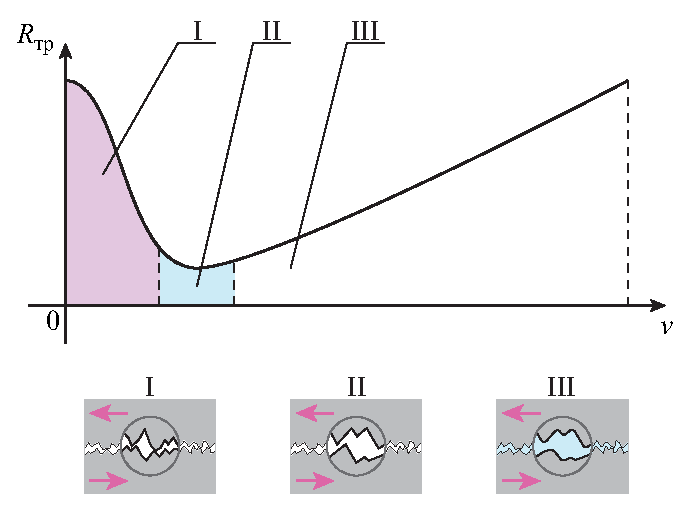
\includegraphics{part2/friction_model_demonstrate.eps}
    }
    \caption{Графическое представление модели трения}
    \label{fig:ch2/friction_model}
\end{figure}

Данная модель позволяет учесть ключевые особенности фрикционного взаимодействия в пневмоприводе:

Рассмотрим каждый компонент модели более подробно:
\begin{enumerate}
    \item Кулоновское трение:
          $$R_\text{к} = \mu_\text{к} N \text{sign}(v)$$
          где $\mu_\text{к}$ - коэффициент кулоновского трения, $N$ - нормальная сила. Кулоновское трение обеспечивает
          постоянную составляющую силы трения при установившемся движении;

    \item Статическое трение:
          $$R_\text{с} = \mu_\text{с} N \text{sign}(R_\text{вн})$$
          где $\mu_\text{с}$ - коэффициент статического трения, $R_\text{вн}$ - внешняя приложенная сила.
          Статическое трение препятствует началу движения при малых управляющих воздействиях;

    \item Эффект Штрибека:
          $$R_\text{ш} = (R_\text{с} - R_\text{к})e^{-\left|\frac{v}{v_\text{ш}}\right|^\delta}$$
          Эффект Штрибека описывает падение силы трения при переходе от состояния покоя к движению;

    \item Вязкое трение:
          $$R_\text{в} = \sigma_2 v$$
          где $\sigma_2$ - коэффициент вязкого трения. Вязкое трение зависит от скорости движения и преобладает при высоких скоростях.

\end{enumerate}

% Для определения параметров статической модели трения применяется следующий подход:

% \begin{enumerate}
%     \item Идентификация $R_\text{к}$ и $R_\text{в}$:
%           Проводятся тесты с постоянной скоростью движения. При установившемся движении сила трения описывается уравнением:
%           $$R_\text{тр} = R_\text{к} \text{sign}(v) + R_\text{в} v$$
%           Линейная регрессия по экспериментальным данным позволяет определить $R_\text{к}$ и $R_\text{в}$;

%     \item Идентификация $R_\text{с}$:
%           $R_\text{с}$ оценивается по максимальному значению силы трения при начале движения:
%           $$R_\text{с} = \max(|R_\text{тр}|) \text{ при } v \approx 0;$$

%     \item Идентификация $v_\text{ш}$ и $\delta$:
%           Параметры $v_\text{ш}$ и $\delta$ определяются путем минимизации среднеквадратичной ошибки между экспериментальной кривой зависимости силы трения от скорости и теоретической кривой:
%           $$\min_{v_\text{ш}, \delta} \sum_{i=1}^N (R_{\text{тр},i}^{\text{эксп}} - R_{\text{тр},i}^{\text{модель}}(v_\text{ш}, \delta))^2$$.
% \end{enumerate}

% Верификация статической модели трения осуществляется путем сравнения результатов моделирования
% с экспериментальными данными, полученными на реальном пневмоприводе. Проводится серия экспериментов
% с различными режимами движения, включая:

% \begin{enumerate}
%     \item Движение с постоянной скоростью;
%     \item Разгон и торможение;
%     \item Реверсивное движение;
%     \item kДвижение с малыми перемещениями.
% \end{enumerate}

% Для каждого эксперимента вычисляется среднеквадратичная ошибка между предсказанными и измеренными значениями силы трения:
% \begin{equation*}
%     RMSE = \sqrt{\frac{1}{N}\sum_{i=1}^N (R_{\text{тр},i}^{\text{эксп}} - R_{\text{тр},i}^{\text{модель}})^2}
% \end{equation*}

% Адекватность модели оценивается по совокупности критериев, включая RMSE, коэффициент
% детерминации $R^2$, и визуальный анализ графиков зависимости силы трения от скорости.
Данная статическая модель трения позволяет учесть основные нелинейные
эффекты фрикционного взаимодействия в пневмоприводе, что критически важно для
точного моделирования и эффективного управления системой. Однако следует отметить, что
статическая модель имеет ограничения в описании некоторых динамических эффектов, таких
как предварительное смещение и гистерезис, которые могут быть
существенными при прецизионном позиционировании.


\section{Моделирование силы реакции опоры}\label{sec:ch2/sec2/subsec5}

В контексте математического моделирования электропневматического привода существенную роль играет
адекватное описание силы реакции опоры. Данная сила возникает при контакте поршня пневмоцилиндра
с ограничителями хода и оказывает значительное влияние на динамику системы, особенно в крайних положениях.

Сила реакции опоры $R_\text{оп}$ может быть представлена как функция положения поршня $x$ и его скорости $\dot{x}$:
\begin{equation*}
    R_\text{оп} = f(x, \dot{x}).
\end{equation*}

При этом необходимо учитывать, что данная сила проявляется только при достижении
поршнем крайних положений. Таким образом, модель силы реакции опоры должна включать
условия её активации.

Наиболее распространенным подходом к моделированию силы реакции опоры является использование кусочно-линейной модели с учетом жесткости и демпфирования. Данная модель может быть описана следующим образом:
\begin{equation}\label{eq:ch2/support_reaction}
    R_\text{оп} = \begin{cases}
        k_\text{оп}(x - x_\text{мин}) + b_\text{оп}\dot{x},  & \text{если } x < x_\text{мин}                       \\
        0,                                                   & \text{если } x_\text{мин} \leq x \leq x_\text{макс} \\
        k_\text{оп}(x - x_\text{макс}) + b_\text{оп}\dot{x}, & \text{если } x > x_\text{макс}
    \end{cases}
\end{equation}

\section{Моделирование дискретных распределителей}\label{sec:ch2/sec3}

\subsection{Уравнения массового расхода рабочего тела}\label{sec:ch2/sec3/subsec1}
Массовый расход воздуха через дискретный распределитель
является ключевым параметром, определяющим динамику пневматической
системы. Для его описания используется модель, основанная на уравнении Сен-Венана-Ванцеля:
\begin{equation}
    G = \psi(p_1, p_2) \cdot u C_d F_e \frac{p_1}{\sqrt{RT_\text{вх}}},
\end{equation}
где
$G$ -- массовый расход воздуха;
$\psi(p_1, p_2)$ -- расходная функция;
$u$ -- положение золотника $(0 \div 1)$;
$C_d$ -- коэффициент расхода;
$F_e$ -- эффективная площадь проходного сечения;
$p_1$ -- давление на входе;
$p_2$ -- давление на выходе;
$R$ -- газовая постоянная для воздуха;
$T_\text{вх}$ -- температура воздуха на входе.

Ключевым элементом в данном уравнении является расходная функция $\psi(p_1, p_2)$, которая
учитывает влияние отношения давлений на входе и выходе распределителя
на массовый расход. Эта функция определяется следующим образом:
\begin{equation*}
    \psi(p_1, p_2) = \begin{cases}
        \sqrt{\frac{2\gamma}{\gamma-1}\left[\left(\frac{p_2}{p_1}\right)^{\frac{2}{\gamma}} - \left(\frac{p_2}{p_1}\right)^{\frac{\gamma+1}{\gamma}}\right]}, & \text{если } \frac{p_2}{p_1} > b_{кр}    \\
        \sqrt{\gamma \left(\frac{2}{\gamma+1}\right)^{\frac{\gamma+1}{\gamma-1}}},                                                                            & \text{если } \frac{p_2}{p_1} \leq b_{кр}
    \end{cases}
\end{equation*}
где
$\gamma$ -- показатель адиабаты для воздуха;
$b_{кр} = \left(\frac{2}{\gamma+1}\right)^{\frac{\gamma}{\gamma-1}}$ -- критическое отношение давлений.

Для наглядного представления характера изменения расходной функции
$\psi(p_1, p_2)$ в зависимости от отношения давлений $p_2/p_1$
приведен график представленны на рисунке \ref{fig:ch2/mass_flow_function}.
\begin{figure}
    \centerfloat{
        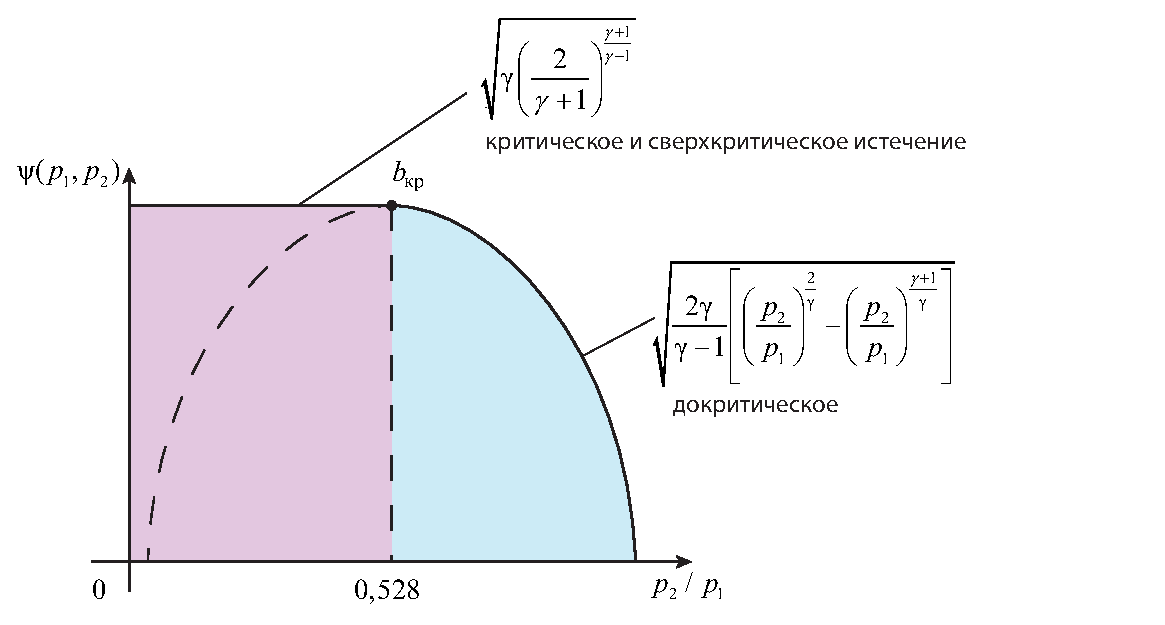
\includegraphics{part2/critical_gas_flow_chart.eps}
    }
    \caption{График расходной функции $\psi(p_1, p_2)$}
    \label{fig:ch2/mass_flow_function}
\end{figure}

На графике отчетливо видны две области: докритическое и закритическое течение, разделенные точкой
критического отношения давлений $b_{кр}$.

В области докритического течения ($p_2/p_1 > b_{кр}$) расход зависит от отношения давлений и
описывается нелинейной функцией. Здесь наблюдается плавное увеличение расхода с уменьшением отношения давлений.

В закритической области ($p_2/p_1 \leq b_{кр}$) расход достигает максимального
значения и остается постоянным независимо от дальнейшего снижения отношения давлений.
Это явление связано с достижением скорости потока воздуха
в самом узком сечении распределителя скорости звука.

Критическая точка $b_{кр}$ соответствует условию, при котором скорость потока
воздуха в самом узком сечении распределителя достигает скорости звука. Для
воздуха при нормальных условиях значение $b_{кр}$ составляет приблизительно \num{0.528}.
Эффективная площадь проходного сечения $F_\text{др}$ зависит от
положения запорно-регулирующего элемента распределителя и может
быть представлена как функция управляющего сигнала $u$:
\begin{equation*}
    F_\text{др} = F_{max} \cdot f(u),
\end{equation*}
где $F_{max}$ -- максимальная эффективная площадь проходного сечения;
$f(u)$ -- функция, описывающая зависимость площади от управляющего сигнала.

Представленная модель массового расхода позволяет точно описать процесс истечения
воздуха через дискретный распределитель в различных режимах работы
пневмопривода. Учет нелинейного характера расходной функции и
влияния критического отношения давлений особенно важен при анализе динамики
системы и разработке алгоритмов управления, обеспечивающих высокую точность
и быстродействие электропневматического привода.

\subsection{Динамика переключения распределителей}\label{sec:ch2/sec3/subsec2}

Процесс переключения дискретного распределителя характеризуется
определенной динамикой, которую необходимо учитывать для точного моделирования поведения
системы. Динамика переключения может быть описана дифференциальным уравнением первого порядка:
\begin{equation}\label{eq:ch2/switching_dynamics}
    \tau \frac{du}{dt} + u = u_{зад},
\end{equation}
где:
$u$ -- текущее положение запорно-регулирующего элемента;
$u_{зад}$ -- заданное положение (0 или 1 для дискретного распределителя);
$\tau$ -- постоянная времени переключения.

Альтернативно, для более точного описания динамики переключения
может быть использована модель второго порядка:
\begin{equation}
    \frac{d^2u}{dt^2} + 2\zeta\omega_n\frac{du}{dt} + \omega_n^2u = \omega_n^2u_{зад}
\end{equation}
где $\zeta$ -- коэффициент демпфирования;
$\omega_n$ -- собственная частота колебаний.

Учет динамики переключения позволяет моделировать такие эффекты, как задержка
срабатывания и дребезг контактов, которые могут оказывать
существенное влияние на поведение системы,
особенно при высокочастотном управлении.

Интеграция моделей массового расхода и динамики переключения
в общую математическую модель электропневматического привода
осуществляется путем их включения в уравнения
изменения давлений в полостях пневмоцилиндра \ref{eq:ch2/eq_pressure_system}.

В данной работе использована модель первого порядка для описания динамики переключения
поскольку она обеспечивает достаточно точное описание процесса переключения
и имеет простую структуру.


\section{Адаптация математической модели к эффективному численному расчету на ЭВМ}\label{sec:ch2/sec5}

Эффективное численное моделирование динамики электропневматического привода требует
оптимизации математической модели для выполнения расчетов на ЭВМ.
Данный этап критически важен для обеспечения высокой производительности
вычислений при проведении многочисленных итераций в задачах оптимизации,
анализа чувствительности и робастности системы управления.

Основные цели оптимизации математической модели включают:

\begin{enumerate}
    \item Снижение вычислительной сложности уравнений;
    \item Уменьшение времени выполнения расчетов;
    \item Повышение численной устойчивости алгоритмов;
    \item Эффективное использование параллельных вычислительных архитектур.
\end{enumerate}

Для достижения этих целей будут применены следующие методы:

\begin{enumerate}
    \item Векторизация уравнений;
    \item Упрощение и линеаризация нелинейных выражений;
    \item Предварительное вычисление констант и коэффициентов;
\end{enumerate}

\subsection{Векторизация уравнений}\label{sec:ch2/sec5/subsec1}
Векторизация уравнений представляет собой эффективный метод оптимизации вычислений,
позволяющий использовать преимущества SIMD-инструкций (Single Instruction, Multiple Data)
современных процессоров. Данный подход особенно актуален для математической
модели электропневматического привода с дискретными распределителями, где многие операции могут быть выполнены
параллельно \cite*{eichenberger2004simd} над несколькими элементами данных.

Основная идея векторизации заключается в преобразовании скалярных операций в
векторные, что позволяет обрабатывать несколько элементов данных
одновременно \cite*{nuzman2011vaporsimd}. В контексте рассматриваемой модели это означает переход от
поэлементных вычислений к операциям над векторами и матрицами.
Процесс векторизации начинается с представления состояния системы
в виде единого вектора. Для электропневматического привода
вектор состояния может быть записан как:

\begin{equation}
    \mathbf{y} = [x, v, p_1, p_2, T_1, T_2, x_{v1}, x_{v2}, x_{v3}, x_{v4}]^T.
\end{equation}

Система дифференциальных уравнений, описывающая динамику привода, преобразуется к векторной форме:
\begin{equation*}
    \frac{d\mathbf{y}}{dt} = \mathbf{f}(\mathbf{y}, t),
\end{equation*}
где $\mathbf{f}$ -- векторная функция, компоненты которой соответствуют правым частям исходных дифференциальных уравнений.

Векторизация уравнений массового расхода через распределители является одним из ключевых
элементов оптимизации. Вместо последовательного расчета расхода для
каждого распределителя, формируется вектор массовых расходов:

\begin{equation*}
    \mathbf{G} = \boldsymbol{\psi}(\mathbf{p}_1, \mathbf{p}_2) \odot \mathbf{u} \odot \mathbf{C}_d \odot \mathbf{F}_\text{др} \odot \frac{\mathbf{p}_{\text{вх}}}{\sqrt{R\mathbf{T}_{\text{вх}}}},
\end{equation*}
где $\odot$ -- поэлементное умножение векторов;
$\boldsymbol{\psi}(\mathbf{p}_1, \mathbf{p}_2)$ -- вектор-функция расходных характеристик;
$\mathbf{u}$ -- вектор управляющих сигналов;
$\mathbf{C}_d$ - вектор коэффициентов расхода;
$\mathbf{F}_\text{др}$ -- вектор эффективных площадей проходных сечений;
$\mathbf{p}_{вх}$ и $\mathbf{T}_{вх}$ -- векторы давлений и температур на входе распределителей соответственно.

Уравнения изменения давления в полостях цилиндра также подвергаются векторизации:

\begin{equation*}
    \frac{d\mathbf{p}}{dt} = \frac{\gamma R}{L} \odot \frac{\mathbf{T}}{\mathbf{V}} \odot
    \left(\mathbf{G}_{\text{вх}} - \mathbf{G}_{\text{вых}} - \frac{\mathbf{p}}{R\mathbf{T}} \odot \frac{d\mathbf{V}}{dt}\right),
\end{equation*}
где $\mathbf{p} = [p_1, p_2]^T$, $\mathbf{T} = [T_1, T_2]^T$, $\mathbf{V} = [V_1/L, V_2/L]^T$ --
векторы давлений, температур и нормализованных объемов полостей соответственно.

Векторизация затрагивает и уравнения изменения температуры в полостях:
\begin{equation*}
    \frac{d\mathbf{T}}{dt} = \frac{\mathbf{T}}{\mathbf{p}} \odot \frac{d\mathbf{p}}{dt} -
    (\gamma - 1) \frac{\mathbf{T}}{\bar{\mathbf{V}}} \odot \frac{d\bar{\mathbf{V}}}{dt}
\end{equation*}

Векторизация расчета расходной функции $\psi(p_1, p_2)$ осуществляется путем применения
векторных операций к отношениям давлений:
\begin{equation*}
    \boldsymbol{\psi}(\mathbf{p}_1, \mathbf{p}_2) = \begin{cases}
        \sqrt{\frac{2\gamma}{\gamma-1}\left[\left(\frac{\mathbf{p}_2}{\mathbf{p}_1}\right)^{\frac{2}{\gamma}} - \left(\frac{\mathbf{p}_2}{\mathbf{p}_1}\right)^{\frac{\gamma+1}{\gamma}}\right]}, & \text{если } \frac{\mathbf{p}2}{\mathbf{p}1} > b{кр},     \\
        \psi{макс},                                                                                                                                                                               & \text{если } \frac{\mathbf{p}_2}{\mathbf{p}1} \leq b{кр},
    \end{cases}
\end{equation*}
где операции возведения в степень и сравнения выполняются поэлементно.

Уравнения димаки золотника распределителей тоже можно векторизовать:
\begin{equation}
    \tau \frac{d\mathbf{u}}{dt} + \mathbf{u} = \mathbf{u}_\text{зад},
\end{equation}
где $\mathbf{u}$ -- вектор управляющих сигналов золотников;
$\mathbf{u}_\text{зад}$ -- вектор заданных значений управляющих сигналов.

Применение векторизации позволяет эффективно использовать SIMD-инструкции процессора,
что приводит к значительному ускорению вычислений. В зависимости от архитектуры процессора и
специфики реализации, ускорение может достигать 2-4 раза \cite*{tian2013simd} по сравнению с исходной скалярной версией.

\subsection{Оптимизация нелинейных функций}\label{sec:ch2/sec5/subsec2}

Так же важным этапом оптимизации является упрощение и линеаризация нелинейных функций,
которые могут оказывать существенное влияние на вычислительную сложность модели и деаль ее
жесткой. В контексте электропневматического привода, к нелинейным функцям относятся экспоненциальная
функция в модели трения, функция sign, реакция упоров и условные операции.

Для оптимизации вычисления экспоненциальной функции в модели трения предлагается использовать аппроксимацию Паде.
Данный метод обеспечивает высокую точность аппроксимации при сравнительно низкой вычислительной
сложности. Аппроксимация Паде для экспоненциальной функции может быть представлена в виде:

\begin{equation*}
    e^x \approx \frac{1 + \frac{x}{2} + \frac{x^2}{10} + \frac{x^3}{120}}{1 - \frac{x}{2} + \frac{x^2}{10} - \frac{x^3}{120}}.
\end{equation*}

Данная аппроксимация обеспечивает высокую точность в диапазоне $x \in [-2,5; 2,5]$,
что достаточно для моделирования эффекта Штрибека в рассматриваемой системе.

Функция sign, используемая в модели трения, может быть аппроксимирована
гладкой функцией для улучшения численной стабильности:

\begin{equation*}
    \text{sign}(x) \approx \tanh(kx),
\end{equation*}

где $k$ -- параметр, определяющий крутизну перехода. Рекомендуется выбирать k в диапазоне
$100 \div 1000$ для баланса между точностью аппроксимации и численной стабильностью.

Реакция упоров, обычно моделируемая с использованием условных операций, может быть
оптимизирована применением непрерывной аппроксимации:

\begin{equation*}
    R_\text{оп} = k_\text{оп}(x - x_\text{мин})\cdot S(x - x_\text{мин}) + k_\text{оп}(x - x_\text{макс})\cdot S(x - x_\text{макс}),
\end{equation*}
где $S(x)$ -- сглаживающая функция, например:

\begin{equation*}
    S(x) = \frac{1}{1 + e^{-\alpha x}},
\end{equation*}
где $\alpha$ -- параметр, определяющий крутизну перехода.

Для оптимизации условных операций в модели предлагается
использовать непрерывные аппроксимации. Например, функция
максимума может быть аппроксимирована как:

\begin{equation*}
    \max(a, b) \approx \frac{a + b + \sqrt{(a - b)^2 + \varepsilon}}{2},
\end{equation*}
где $\varepsilon$ -- малое положительное число, обеспечивающее гладкость функции.

Применяя предложенные оптимизации, уравнения реакции упоров и силы трения могут быть представлены в виде:

\begin{equation}
    \begin{alignedat}{2}
        R_\text{тр} & = \left[R_\text{к} + (R_\text{с} - R_\text{к})\frac{1 + \frac{z}{2} + \frac{z^2}{10} + \frac{z^3}{120}}{1 - \frac{z}{2} + \frac{z^2}{10} - \frac{z^3}{120}}\right]\tanh(k\dot{x}) + R_\text{в}\dot{x}, \\
        R_\text{оп} & = k_\text{оп}(x - x_\text{мин})\cdot \frac{1}{1 + e^{-\alpha(x - x_\text{мин})}} + k_\text{оп}(x - x_\text{макс})\cdot \frac{1}{1 + e^{-\alpha(x - x_\text{макс})}},
    \end{alignedat}
\end{equation}

\subsection{Аналитическое вычисление якобиана для численного решения ОДУ}\label{sec:ch2/sec5/subsec3}
Так же в рамках оптимизации модели использовалось аналитическое вычисление якобиана для
решателей ОДУ, что позволяет уменьшить количество вычислений и повысить численную стабильность.

Якобиан системы определяется как матрица частных производных:

\begin{equation}\label{eq:ch2/jacobian}
    J = \frac{\partial \mathbf{f}}{\partial \mathbf{y}} =
    \begin{pmatrix}
        \frac{\partial f_1}{\partial y_1}    & \frac{\partial f_1}{\partial y_2}    & \cdots & \frac{\partial f_1}{\partial y_{10}}    \\
        \frac{\partial f_2}{\partial y_1}    & \frac{\partial f_2}{\partial y_2}    & \cdots & \frac{\partial f_2}{\partial y_{10}}    \\
        \vdots                               & \vdots                               & \ddots & \vdots                                  \\
        \frac{\partial f_{10}}{\partial y_1} & \frac{\partial f_{10}}{\partial y_2} & \cdots & \frac{\partial f_{10}}{\partial y_{10}}
    \end{pmatrix}
\end{equation}

где $\mathbf{f}$ -- вектор-функция правых частей системы дифференциальных уравнений.

Ключевые элементы якобиана включают:
\begin{enumerate}
    \item Частные производные уравнения движения поршня:
          \begin{equation*}
              \begin{alignedat}{2}
                  \frac{\partial \dot{x}}{\partial x}   & = 0, & \quad \frac{\partial \dot{x}}{\partial v}   & = 1,                     \\
                  \frac{\partial \dot{v}}{\partial x}   & = 0, & \quad \frac{\partial \dot{v}}{\partial v}   & =
                  \frac{1}{M}(\mathbf{p}^T\mathbf{F} - p_\text{атм}(\mathbf{1}^T\mathbf{F}) - R_\text{тр} - R_\text{оп} - R_\text{вн}), \\
                  \frac{\partial \dot{v}}{\partial p_1} & = 0, & \quad \frac{\partial \dot{v}}{\partial p_2} & = 0.
              \end{alignedat}
          \end{equation*}

    \item Частные производные уравнений изменения давления:
          \begin{equation*}
              \begin{alignedat}{2}
                  \frac{\partial \dot{p}_i}{\partial x}    & = -\gamma p_i A_i / V_i,                                                           \\
                  \frac{\partial \dot{p}_i}{\partial v}    & = -\gamma p_i A_i / V_i,                                                           \\
                  \frac{\partial \dot{p}_i}{\partial p_i}  & = \gamma \left(R T_i \frac{\partial \dot{m}_i}{\partial p_i} - A_i v\right) / V_i, \\
                  \frac{\partial \dot{p}_i}{\partial T_i}  & = \gamma R \dot{m}_i / V_i,                                                        \\
                  \frac{\partial \dot{p}i}{\partial x{vj}} & = \gamma R T_i \frac{\partial \dot{m}i}{\partial x{vj}} / V_i;
              \end{alignedat}
          \end{equation*}

    \item Частные производные уравнений изменения температуры:

          \begin{equation*}
              \frac{\partial \dot{T}_i}{\partial y_j} = \frac{T_i}{p_i}\frac{\partial \dot{p}_i}{\partial y_j}
              - (\gamma - 1)\frac{T_i}{V_i}\frac{\partial \dot{V}_i}{\partial y_j};
          \end{equation*}
    \item Частные производные уравнений динамики золотников:
          \begin{equation*}
              \frac{\partial \dot{x}_{vi}}{\partial x_{vi}} = -1/\tau;
          \end{equation*}
\end{enumerate}

Запишем полный якобиан \ref{eq:ch2/jacobian} системы:

\begin{equation*}
    J = \begin{bmatrix}
        J_{xx}  & J_{xv}  & J_{xp}  & J_{xT}  & J_{xxv}  \\
        J_{vx}  & J_{vv}  & J_{vp}  & J_{vT}  & J_{vxv}  \\
        J_{px}  & J_{pv}  & J_{pp}  & J_{pT}  & J_{pxv}  \\
        J_{Tx}  & J_{Tv}  & J_{Tp}  & J_{TT}  & J_{Txv}  \\
        J_{xvx} & J_{xvv} & J_{xvp} & J_{xvT} & J_{xvxv}
    \end{bmatrix},
\end{equation*}

в данной матрице якобина каждый блок представляет собой подматрицу частных производных.
Рассмотрим каждый блок подробнее:
\begin{enumerate}
    \item $J_{xx}$ -- матрица размером $2 \times 2$
          \begin{equation*}
              J_{xx} = \begin{bmatrix}
                  0                                         & 1 \\
                  \frac{\partial F_\text{тр}}{\partial x}/M & 0
              \end{bmatrix};
          \end{equation*}

    \item $J_{xv}$ -- матрица размером $2 \times 2$
          \begin{equation*}
              J_{xv} = \begin{bmatrix}
                  0 & 0                                                                                                     \\
                  0 & \left( \frac{\partial F_\text{тр}}{\partial v}/M  + \frac{\partial F_\text{оп}}{\partial v}/M \right)
              \end{bmatrix};
          \end{equation*}

    \item $J_{xp}$ -- матрица размером $2 \times 2$
          \begin{equation*}
              J_{xp} = \begin{bmatrix}
                  0     & 0      \\
                  F_1/M & -F_2/M
              \end{bmatrix}
          \end{equation*};

    \item $J_{xT}$ -- матрица $O_{2,2}$;

    \item $J_{xxv}$ -- матрица $O_{3,3}$;

    \item $J_{vx} = J_{xv}^T$;

    \item $J_{vv} = J_{xv}$;

    \item $J_{vp} = J_{xp}$;

    \item $J_{vT} = J_{xT}$;

    \item $J_{vxv} = J_{xxv}$

    \item $J_{px}$ -- матрица размером $2 \times 2$
          \begin{equation*}
              J_{px} = \begin{bmatrix}
                  -\gamma p_1 F_1 / V_1 & -\gamma p_1 F_1 / V_1 \\
                  \gamma p_2 F_2 / V_2  & \gamma p_2 F_2 / V_2
              \end{bmatrix};
          \end{equation*}

    \item $J_{pv} = J_{px}$;

    \item $J_{pp}$ -- матрица размером $2 \times 2$
          \begin{equation*}
              J_{pp} = \begin{bmatrix}
                  \gamma R T_1 \frac{\partial \dot{m}_1}{\partial p_1} - F_1 v / V_1 & 0                                                                  \\
                  \0                                                                 & \gamma R T_2 \frac{\partial \dot{m}_2}{\partial p_2} - F_2 v / V_2
              \end{bmatrix};
          \end{equation*}

    \item $J_{pT}$ -- матрица размером $2 \times 2$

          \begin{equation*}
              J_{pT} = \begin{bmatrix}
                  \gamma R \dot{m}_1 / V_1 & 0                        \\
                  0                        & \gamma R \dot{m}_2 / V_2
              \end{bmatrix};
          \end{equation*}

    \item $J_{pxv}$ -- матрица размером $4 \times 2$

          \begin{equation*}
              J_{pxv} = \begin{bmatrix}
                  \gamma R T_1 \frac{\partial \dot{m}_1}{\partial x_{v1}}/V_1 & -\gamma R T_1 \frac{\partial \dot{m}_1}{\partial x_{v2}}/V_1 & 0                                                           & 0                                                            \\
                  0                                                           & 0                                                            & \gamma R T_2 \frac{\partial \dot{m}_2}{\partial x_{v3}}/V_2 & -\gamma R T_2 \frac{\partial \dot{m}_2}{\partial x_{v4}}/V_2
              \end{bmatrix};
          \end{equation*}

    \item $J_{Tx}$ -- матрица размером $2 \times 2$
          \begin{equation*}
              J_{Tx} = \begin{bmatrix}
                  T_1 J_{px,11}/p_1 & T_1 J_{px,12}/p_1 \\
                  T_2 J_{px,21}/p_2 & T_2 J_{px,22}/p_2
              \end{bmatrix};
          \end{equation*}

    \item $J_{Tv} = J_{Tx}$;

    \item $J_{Tp}$ -- матрица размером $2 \times 2$
          \begin{equation*}
              J_{Tp} = \begin{bmatrix}
                  T_1 J_{pp,11}/p_1 & 0                 \\
                  0                 & T_2 J_{pp,22}/p_2
              \end{bmatrix};
          \end{equation*}

    \item $J_{TT}$ -- матрица размером $2 \times 2$
          \begin{equation*}
              J_{TT} = \begin{bmatrix}
                  J_{pp,11} T_1/p_1 & 0                 \\
                  0                 & J_{pp,22} T_2/p_2
              \end{bmatrix};
          \end{equation*}

    \item $J_{Txv}$ -- матрица размером $3 \times 2$
          \begin{equation*}
              J_{Txv} = \begin{bmatrix}
                  T_1 J_{pxv,11}/p_1 & T_1 J_{pxv,12}/p_1 & 0                  & 0                  \\
                  0                  & 0                  & T_2 J_{pxv,23}/p_2 & T_2 J_{pxv,24}/p_2
              \end{bmatrix};
          \end{equation*}

    \item $J_{xvx} = J_{xvv} = J{xvp} = J_{xvT}$ -- матрица $O_{2,4}$;

    \item $J_{xvxv}$ -- матрица размером $4 \times 4$
          \begin{equation*}
              J_{xvxv} = \begin{bmatrix}
                  -1/\tau & 0       & 0       & 0       \\
                  0       & -1/\tau & 0       & 0       \\
                  0       & 0       & -1/\tau & 0       \\
                  0       & 0       & 0       & -1/\tau
              \end{bmatrix};
          \end{equation*}
\end{enumerate}

Применение якобиана для в методах численных численного интегрирования, таких как
BDF (Backward Differentiation Formula) и Radau, позволяет уменьшить количество вычислений
и повысить численную стабильность. В частности, использование якобиана позволяет
уменьшить количество вычислений правых частей системы, что особенно важно для жестких систем.

\section{Реализация математической модели}\label{sec:ch2/sec6}

Сведем полученные выражения в единую систему:

\begin{equation}
    \begin{cases}
        \begin{alignedat}{2}
            \frac{dx}{dt}          & = v                                                                                                                                                                                                    \\
            \frac{dv}{dt}          & = \frac{1}{M}(\mathbf{p}^T\mathbf{F} - p_\text{атм}(\mathbf{1}^T\mathbf{F}) - R_\text{тр} - R_\text{оп} - R_\text{вн} )                                                                                \\                                                                                                                   \\
            \frac{d\mathbf{p}}{dt} & = \frac{\gamma R}{L} \odot \frac{\mathbf{T}}{\bar{\mathbf{V}}} \odot \left(\mathbf{G}_{\text{вх}} - \mathbf{G}_{\text{вых}} - \frac{\mathbf{p}}{R\mathbf{T}} \odot \frac{d\bar{\mathbf{V}}}{dt}\right) \\
            \frac{d\mathbf{T}}{dt} & = \frac{\mathbf{T}}{\mathbf{p}} \odot \frac{d\mathbf{p}}{dt} - (\gamma - 1) \frac{\mathbf{T}}{\bar{\mathbf{V}}} \odot \frac{d\bar{\mathbf{V}}}{dt}                                                     \\
            \mathbf{G}             & = \boldsymbol{\psi}(\mathbf{p}_1, \mathbf{p}_2) \odot \mathbf{u} \odot \mathbf{C}_d \odot \mathbf{F}_\text{др} \odot \frac{\mathbf{p}_{\text{вх}}}{\sqrt{R\mathbf{T}_\text{вх}}}                       \\
            R_\text{тр}            & = \left[R_\text{к} + (R_\text{с} - R_\text{к})\frac{1 + \frac{z}{2} + \frac{z^2}{10} + \frac{z^3}{120}}{1 - \frac{z}{2} + \frac{z^2}{10} - \frac{z^3}{120}}\right]\tanh(k\dot{x}) + R_\text{в}\dot{x}  \\
            R_\text{оп}            & = k_\text{оп}(x - x_\text{мин})\cdot \frac{1}{1 + e^{-\alpha(x - x_\text{мин})}} + k_\text{оп}(x - x_\text{макс})\cdot \frac{1}{1 + e^{-\alpha(x - x_\text{макс})}}                                    \\
            \mathbf{u}_\text{зад}  & = \tau \frac{d\mathbf{u}}{dt} + \mathbf{u}
        \end{alignedat}
    \end{cases}
\end{equation}
где
$\mathbf{p} = [p_1, p_2]^T$ -- вектор давлений в полостях цилиндра;
$\mathbf{F} = [F_1, -F_2]^T$ -- вектор эффективных площадей поршня;
$\mathbf{1} = [1, 1]^T$ -- единичный вектор;
$p_\text{атм}$ -- атмосферное давление (скалярная величина);
$(\mathbf{1}^T\mathbf{F}) = F_1 - F_2$ -- результат векторного произведения, дающий разность площадей;
$\mathbf{u}$ -- вектор управляющих сигналов золотников;
$\mathbf{u}_\text{зад}$ -- вектор заданных значений управляющих сигналов;

Реализация математической модели электропневматического привода осуществляется с использованием языка программирования Python
и специализированных библиотек для научных вычислений. Основой реализации служит класс \texttt{ElectroPneumaticActuator},
который инкапсулирует параметры системы и методы для моделирования ее динамики.

Структура класса включает конструктор для инициализации параметров привода, методы для расчета производных состояния системы,
а также вспомогательные функции для вычисления отдельных компонентов модели, таких как массовые расходы, силы трения и реакции упоров.
Ключевым элементом реализации является метод \texttt{calculate\_derivatives}, который формирует систему дифференциальных уравнений,
описывающих динамику привода.

\begin{ListingEnv}[!h]% настройки floating аналогичны окружению figure
    \captiondelim{ } % разделитель идентификатора с номером от наименования
    \caption{ \protect\python}\label{lst:hwbeauty}
    % окружение учитывает пробелы и табуляции и применяет их в сответсвии с настройками
    \begin{lstlisting}[language={Python}]
import numpy as np
from scipy.integrate import solve_ivp
from numba import njit

class ElectroPneumaticActuator:
    def __init__(self, params):
        self.m = params['m']  # Масса подвижных частей
        self.A1 = params['A1']  # Эффективная площадь поршня со стороны штока
        # Остальные параметры...

    @njit
    def calculate_derivatives(self, t, y, u):
        x, v, p1, p2, T1, T2 = y

        V1 = self.V0 + self.A1 * x
        V2 = self.V0 + self.A2 * (self.L - x)
        # Расчет отсальных состояний...
        return np.array([dx, dv, dp1, dp2, dT1, dT2])

    @njit
    def mass_flow(self, p_up, p_down, T_up, u):
        # Реализация расчета массового расхода...
    # Реализация остальных методов...

    def solve(self, t_span, y0, u_func):
        sol = solve_ivp(
            lambda t, y: self.calculate_derivatives(t, y, u_func(t)),
            t_span, y0, method='RK45', rtol=1e-6, atol=1e-9
        )
        return sol
    \end{lstlisting}
\end{ListingEnv}%

Центральным элементом модели, как было сказано выше, является метод \texttt{calculate\_derivatives},
который формирует систему дифференциальных уравнений, описывающих динамику привода.
Этот метод учитывает изменение объемов полостей цилиндра, массовые расходы через
распределители, силы, действующие на поршень, и термодинамические процессы в системе.

Метод \texttt{solve} обеспечивает интеграцию различных алгоритмов управления в процесс моделирования,
что позволяет проводить сравнительный анализ эффективности различных стратегий управления приводом.

Полная реализация модели, включая детальные расчеты массовых расходов, сил трения и
различных алгоритмов управления, представлена в приложении к диссертации \fixme{организовать приложение}.

Управление приводом, согласно вышенаписанному, осуществляется путем задания управляющего сигнала $\mathbf{u}$,
который представляет собой вектор состояний дискретных распределителей. Поскольку в рассматриваемой системе используется четыре распределителя, то $\mathbf{u} \in {0,1}^4$, где 0 соответствует
закрытому состоянию распределителя, а 1 -- открытому.

Для реализации различных алгоритмов управления в модель введен абстрактный базовый класс~\texttt{AbstractController},
от которого наследуются конкретные реализации контроллеров. Этот подход обеспечивает гибкость при исследовании
и сравнении различных стратегий управления. Структура класса AbstractController определена следующим образом:

\begin{ListingEnv}[!h]% настройки floating аналогичны окружению figure
    \captiondelim{ } % разделитель идентификатора с номером от наименования
    \caption{ \protect\python}\label{lst:AbstractControllerClass}
    \begin{lstlisting}[language={Python}]
from abc import ABC, abstractmethod

class AbstractController(ABC):
    @abstractmethod
    def calculate_control(self, t, y, y_ref):
        pass

    @abstractmethod
    def convert_to_valve_states(self, u):
        pass
    \end{lstlisting}
\end{ListingEnv}%

Метод \textttt{calculate\_control} вычисляет управляющее воздействие на основе текущего состояния системы \texttt{y},
заданного значения \texttt{y\_ref} и времени \texttt{t}.
Метод \texttt{conver\_to\_valve\_states} преобразует вычисленное управляющее воздействие
в конкретные состояния распределителей.

\section{Верификация математической модели}\label{sec:ch2/sec7}
Верификация математической модели  представляет собой неотъемлемый этап разработки, направленный на подтверждение адекватности
и точности полученного математического описания. Процесс верификации включает в себя комплекс методов и подходов,
позволяющих оценить соответствие модели реальному объекту в рамках принятых допущений и ограничений.

Основной целью верификации является подтверждение способности модели корректно отражать физические процессы,
происходящие в электропневматическом приводе, и обеспечивать достоверные результаты при решении задач анализа и синтеза систем управления.
В отсутствие экспериментальных данных, предварительная верификация базируется на теоретическом анализе,
численном моделировании.

Верификация данных происходила на основе следующих параметров модели, которые согласованны
с характерными параметрами экпериментального стенда и пердставлены в
таблице \ref{tab:ch2/extended_parameters}.

\begin{table}[h]
    \centering
    \caption{Расширенные параметры моделирования электропневматического привода}
    \small
    \begin{tabular}{lccl}
        \textbf{Параметр}                & \textbf{Обозначение}                      & \textbf{Значение}     & \textbf{Размерность} \\
        \midrule
        Масса подвижных частей           & $M$                                       & 6.0                   & кг                   \\
        Ход поршня                       & $L$                                       & 0.3                   & м                    \\
        Диаметр поршня                   & $D_\text{п}$                              & 0.032                 & м                    \\
        Диаметр штока                    & $d_\text{шт}$                             & 0.012                 & м                    \\
        Площадь поршня со стороны штока  & $F_2 = \pi(D_\text{п}^2-d_\text{шт}^2)/4$ & $7.07 \times 10^{-4}$ & м$^2$                \\
        Площадь поршня со стороны крышки & $F_1 = \pi D_\text{п}^2/4$                & $8.04 \times 10^{-4}$ & м$^2$                \\
        Давление питания                 & $p_\text{п}$                              & $6 \times 10^5$       & Па                   \\
        Атмосферное давление             & $p_\text{атм}$                            & $1 \times 10^5$       & Па                   \\
        Газовая постоянная воздуха       & $R$                                       & 287                   & Дж/(кг$\cdot$К)      \\
        Температура воздуха              & $T_\text{атм}$                            & 293                   & К                    \\
        Показатель адиабаты              & $\gamma$                                  & 1.4                   & -                    \\
        Коэффициент расхода              & $C_d$                                     & 0.7                   & -                    \\
        Эффективная площадь клапана      & $A_v$                                     & $1.2 \times 10^{-6}$  & м$^2$                \\
        \midrule
        \multicolumn{4}{l}{\textbf{Параметры силы трения:}}                                                                         \\
        \midrule
        Сила сухого трения               & $F_c$                                     & 50                    & Н                    \\
        Сила трения покоя                & $F_s$                                     & 60                    & Н                    \\
        Коэффициент вязкого трения       & $\sigma_2$                                & 100                   & Н$\cdot$с/м          \\
        Скорость Штрибека                & $v_s$                                     & 0.01                  & м/с                  \\
        Показатель степени Штрибека      & $\delta$                                  & 2                     & -                    \\
        \midrule
        \multicolumn{4}{l}{\textbf{Параметры реакции опор:}}                                                                        \\
        \midrule
        Коэффициент жесткости опоры      & $k_\text{оп}$                             & $1 \times 10^6$       & Н/м                  \\
        Коэффициент демпфирования опоры  & $b_\text{оп}$                             & 1000                  & Н$\cdot$с/м          \\
        Координата нижнего упора         & $x_\text{мин}$                            & 0                     & м                    \\
        Координата верхнего упора        & $x_\text{макс}$                           & 0.3                   & м                    \\
        \midrule
    \end{tabular}
    \label{tab:ch2/extended_parameters}
\end{table}

\subsection{Теоретические основы верификкаци}\label{sec:ch2/sec7/subsec1}
Процесс верификации основывается на следующих ключевых принципах:

\begin{enumerate}
    \item Принцип физической непротиворечивости, требующий соответствия модели фундаментальным законам механики и пневматики;
    \item Принцип математической корректности, предполагающий отсутствие ошибок в формулировке уравнений и их решении;
    \item Принцип консервативности, обеспечивающий выполнение законов сохранения массы и энергии в модели;
    \item Принцип устойчивости решения, гарантирующий сходимость численных методов при различных начальных условиях и параметрах системы.
\end{enumerate}

Методологический базис верификации включает:

\begin{enumerate}
    \item Аналитический анализ структуры модели и ее соответствия физическим законам;
    \item Численное моделирование с исследованием сходимости и устойчивости решения;
    \item Анализ предельных случаев и упрощенных режимов работы системы;
    \item Оценку чувствительности модели к вариациям параметров.
\end{enumerate}

Математически процесс верификации может быть формализован как задача минимизации функционала
ошибки между результатами моделирования и теоретическими предсказаниями для известных частных случаев:
\begin{equation*}
    J = \min_{\theta} \sum_{i=1}^{N} \left| f_{\text{модель}}(x_i, \theta) - f_{\text{теория}}(x_i) \right|^2,
\end{equation*}
где $f_{\text{модель}}$ -- функция, описывающая выход модели;
$f_{\text{теория}}$ -- теоретически предсказанное значение;
$x_i$ -- входные параметры;
$\theta$ -- параметры модели;
$N$ -- количество точек сравнения.

Выбор методов верификации обусловлен спецификой исследуемой системы и включает:

\begin{enumerate}
    \item Проверку размерностей и единиц измерения всех величин в уравнениях модели.
    \item    Анализ асимптотического поведения модели при предельных значениях параметров.
    \item Исследование сходимости численного решения при измельчении шага интегрирования.
    \item Оценку энергетического баланса системы и соблюдения закона сохранения массы.
\end{enumerate}

\subsection{Проверка маетматической корректности}\label{sec:ch2/sec7/subsec2}

Проверка математической корректности модели электропневматического привода с дискретными распределителями осуществляется посредством следующих процедур:

\begin{enumerate}
    \item Анализ размерностей и единиц измерения;
    \item Верификация согласованности уравнений с законами сохранения;
    \item Оценка физической непротиворечивости уравнений;
    \item Проверка граничных условий и начальных значений;
    \item Анализ непрерывности и дифференцируемости функций.
\end{enumerate}

Каждая процедура направлена на выявление потенциальных ошибок в математическом описании
системы и обеспечение соответствия модели фундаментальным физическим принципам.

Основыне этапы проверки математической корректности модели подробнее:

\paragraph{Анализ размерностей и единиц измерения.}

Проверка согласованности размерностей всех величин, входящих в уравнения модели, осуществляется с использованием метода анализа размерностей. Для каждого уравнения модели выполняется проверка:
\begin{equation*}
    [LHS] = [RHS],
\end{equation*}
где $[LHS]$ и $[RHS]$ -- размерности левой и правой частей уравнения соответственно.

\paragraph{Верификация согласованности уравнений с законами сохранения.}

Проверяется выполнение законов сохранения массы и энергии. Для закона сохранения массы в пневматической системе:
\begin{equation*}
    \frac{d}{dt}\int_V \rho dV + \oint_S \rho \mathbf{v} \cdot d\mathbf{S} = 0,
\end{equation*}
где $\rho$ -- плотность воздуха; $V$ -- объем системы; $\mathbf{v}$ -- скорость потока; $S$ -- поверхность контрольного объема.

Для закона сохранения энергии:
\begin{equation*}
    \frac{d}{dt}(E_k + E_p + U) = W_{\text{внеш}} - Q
\end{equation*}
где $E_k$ -- кинетическая энергия;
$E_p$ -- потенциальная энергия;
$U$ -- внутренняя энергия;
$W_{\text{внеш}}$ -- работа внешних сил;
$Q$ -- теплота, переданная системе.

\paragraph{Оценка физической непротиворечивости уравнений.}

В рамках оценки физической непротиворечивости уравнений проводится проверка
выполнения второго закона термодинамики для адиабатного процесса, в частности, принципа неубывания энтропии.

Для адиабатной системы изменение энтропии должно удовлетворять неравенству:
\begin{equation*}
    \Delta S \geq 0
\end{equation*}
где $\Delta S$ -- изменение энтропии системы.

Проверка неубывания энтропии осуществляется следующим образом:

\begin{enumerate}
    \item Вычисление изменения энтропии для каждой полости цилиндра на каждом шаге интегрирования:
          \begin{equation*}
              \Delta S_i = m_i c_v \ln\left(\frac{T_{i,k+1}}{T_{i,k}}\right) + m_i R \ln\left(\frac{V_{i,k+1}}{V_{i,k}}\right),
          \end{equation*}
          где $m_i$ -- масса газа в i-й полости;
          $c_v$ -- удельная теплоемкость при постоянном объеме;
          $T_{i,k}$ и $V_{i,k}$ -- температура и объем i-й полости на k-м шаге интегрирования.

    \item Расчет производства энтропии за счет необратимых процессов, включая трение и дросселирование газа:
          \begin{equation*}
              \Delta S_{\text{irr}} = \frac{F_{\text{тр}} \Delta x}{T_{\text{ср}}} + \sum_j G_j R \ln\left(\frac{p_{\text{вых},j}}{p_{\text{вх},j}}\right),
          \end{equation*}
          где $F_{\text{тр}}$ -- сила трения;
          $\Delta x$ -- перемещение;
          $T_{\text{ср}}$ -- средняя температура;
          $G_j$ -- массовый расход через j-й распределитель;
          $p_{\text{вх},j}$ и $p_{\text{вых},j}$ -- давления на входе и выходе j-го распределителя.

    \item Проверка условия неубывания суммарной энтропии системы:
          \begin{equation*}
              \Delta S_{\text{total}} = \sum_i \Delta S_i + \Delta S_{\text{irr}} \geq 0.
          \end{equation*}
\end{enumerate}

Дополнительно проверяется выполнение уравнения адиабатного процесса для каждой полости:
\begin{equation*}
    pV^{\gamma} = \text{const}.
\end{equation*}

\paragraph{Проверка граничных условий и начальных значений.}

Осуществляется верификация корректности заданных граничных условий и начальных значений.
Для пневматической системы это включает проверку согласованности давлений на границах системы:
\begin{equation*}
    p_{\text{вх}} \geq p_i \geq p_{\text{вых}},
\end{equation*}
где $p_{\text{вх}}$ -- давление источника;
$p_i$ - давление в i-й полости;
$p_{\text{вых}}$ -- давление на выходе (обычно атмосферное).

\paragraph{Анализ непрерывности и дифференцируемости функций.}

Проверяется непрерывность и дифференцируемость всех функций, входящих в модель, особенно в точках переключения
режимов работы распределителей. Для функции расхода через распределитель $G(p_1, p_2)$ должно выполняться условие:
\begin{equation*}
    \lim_{p_2 \to p_1^-} G(p_1, p_2) = \lim_{p_2 \to p_1^+} G(p_1, p_2)
\end{equation*}

\subsection{Анализ предельных случаев}\label{sec:ch2/sec7/subsec3}

Анализ предлельных случаев позволяет оценить корректность поведения модели в экстремальных условиях
и проверить соответствие результатов теоретическим предсказаниям.

В рамках исследования предельных случаев рассматриваются следующие аспекты:

\paragraph{Поведение системы при экстремальных значениях параметров.}

Проводится серия численных экспериментов с использованием разработанной математической модели
при предельных значениях ключевых параметров системы. К таким параметрам относятся:
\begin{itemize}
    \item Давление питания $p_s$:
          При $p_s \rightarrow 0$ ожидается отсутствие движения поршня.
          При $p_s \rightarrow \infty$ следует наблюдать ограничение скорости движения поршня, обусловленное силами трения и инерцией.
    \item Масса подвижных частей $m$:
          При $M \rightarrow 0$ динамика системы должна определяться преимущественно силами трения.
          При $M \rightarrow \infty$ ожидается значительное замедление движения поршня.
    \item Коэффициенты трения:
          При стремлении коэффициентов трения к нулю система должна демонстрировать колебательное поведение с минимальным затуханием.
          При значительном увеличении коэффициентов трения ожидается апериодический характер движения с возможным возникновением эффекта "прилипания-скольжения".
    \item Эффективные площади проходных сечений распределителей:
          При $F_\text{др} \rightarrow 0$ должно наблюдаться существенное замедление динамики системы.
          При $F_\text{др} \rightarrow \infty$ ожидается приближение характеристик системы к случаю с идеальным источником давления.
\end{itemize}

\subsection{Оценка физичности результатов моделирования}\label{sec:ch2/sec7/subsec4}

\paragraph{Проверка размерностей и единиц измерения.}
Рассматриваются размерности основных физических величин, используемых в модели:

\begin{itemize}
    \item Длина: $ [L] = \text{м}$;
    \item Время: $ [T] = \text{с}$;
    \item Масса: $ [M] = \text{кг}$;
    \item Сила: $ [F] = \text{кг}\cdot\text{м}/\text{с}^2$;
    \item Давление: $ [P] = \text{кг}/(\text{м}\cdot\text{с}^2)$;
    \item Температура: $ [\Theta] = \text{К}$.
\end{itemize}}

Анализ размерностей для каждого уравнения системы:
\begin{itemize}
    \item Уравнение движения поршня: $ [M\cdot L/T^2] = [P\cdot L^2] + [F]$;
    \item Уравнение изменения давления: $ [P/T] = [M/(L^2\cdot T^2)] $;
    \item Уравнение изменения температуры: $ [\Theta/T] = [\Theta/T]$;
    \item Уравнение массового расхода: $  [M/T] = [L^2] \cdot [P] / [L/T] = [M/T] $;
    \item Уравнение силы трения: $  [F] = [F] + [F\cdot T/L] \cdot [L/T] = [F] $;
    \item Уравнение реакции опоры: $  [F] = [F/L] \cdot [L] = [F] $;
    \item Уравнение динамики золотников: $  [1] = [1]$.
\end{itemize}

Проведенный анализ подтверждает согласованность размерностей во всех уравнениях математической модели.
Это свидетельствует о корректности формулировки модели с точки зрения физических единиц измерения.

\subsection{Заключение о достоверности модели}\label{sec:ch2/sec7/subsec5}
